% ----- CHAPTER 4: AN ALGORITHM TO COMPUTE RANK ----- %

%%%%%%%%%%%%%%%%%%%%%%%%%%%
\section{Proof of the Main Theorem}\label{sec:main_thrm_proof}

In this section we prove Theorem \ref{thm:main_theorem}: specifically, that Algorithm \ref{algo:compute_rank} is guaranteed, assuming BSD and ABC and optionally GRH, to correctly output an elliptic curve's rank in time $\softO(\sqrt{N_E})$, where $N_E$ is the conductor of the input curve. Note that the proof will quote certain results established later in this work. \\

The following precision theorem establishes how many bits precision are needed to provably determine if a given $L$-function Taylor coefficient is zero or not:
\begin{theorem}[BSD, ABC, (GRH)]
\label{prop:k_bits_for_leading_coeff}
Let $E$ have $L$-function $\Les$, conductor $N_E$ and real period $\Omega_E$, and let
\begin{equation}\label{eqn:num_bits_without_GRH}
k = \left\lceil 34 + 3.86 \log_2 N_E + \log_2(\Gamma(1.8 + 1.25\log_2 N_E)) - \log_2 \Omega_E \right\rceil.
\end{equation}
Assuming BSD and ABC, we have the following:
\begin{enumerate}
\item $k = O((\log N_E)^{1+\epsilon})$ for any $\epsilon>0$.
\item If $L_E^{(m)}(1)=0$ for all $0 \le m < n$ and $\frac{L_E^{(n)}(1)}{n!}$ is zero to $k$ bits precision, then $L_E^{(n)}(1)$ is identically zero.
\end{enumerate}
\end{theorem}
If one further assumes GRH, we may instead let
\begin{equation}\label{eqn:num_bits_with_GRH}
k = \left\lceil 22 + 2.47 \log_2 N_E + \log_2(\Gamma(1.25 + 0.87 \log_2 N_E)) - \log_2 \Omega_E \right\rceil
\end{equation}
for the same results to hold.
\begin{proof}
The first statement follows from Theorem \ref{thm:real_period_lower_bound}, which states that $\Omega_E$ is bounded away from zero by a negative power of $N_E$. Also note that $\Gamma(s) = O(e^{s \log s})$, so \\
$\log_2(\Gamma(1.8 + 1.25\log_2 N_E)) = O(\log N_E \log\log N_E)$, from which the result follows.\\

To prove the second statement, observe that by BSD the leading non-zero Taylor coefficient of $\Les$ at the central point is given by Equation \ref{eqn:BSD_formula}. We thus have that
\begin{equation}
C_E\pr \ge \frac{1}{256} \cdot  \Reg_E \cdot\, \Omega_E,
\end{equation}
since $\prod_p c_p \ge 1$, $\# \Sha_E \ge 1$, and by Mazur's Theorem $\# E_{\text{Tor}} \le 16$. Thus
\begin{equation}
\log_2 C_E\pr \ge -16 + \log_2 \Reg_E + \log_2 \Omega_E.
\end{equation}
Now by Theorem \ref{thm:regulator_lower_bound} we have that $\Reg_E \ge 4.36 \times 10^{-6} \cdot (N_E)^{-3.86} \cdot \Gamma(1.8+0.25 \log N_E)^{-1}$. Thus 
$\log_2 \Reg_E \ge  -17.81 - 3.86 \log_2 N_E - \log_2(\Gamma(1.8 + 1.25\log_2 N_E))$, where we have changed the log inside the Gamma factor to base to for consistency with the rest of the logs). We therefore have that
\begin{equation}
\log_2 C_E\pr \ge -33.81 - 3.86 \log_2 N_E - \log_2(\Gamma(1.8 + 1.25\log_2 N_E)) + \log_2 \Omega_E > -k,
\end{equation}
where $k$ is as defined above. Hence if the $n$th taylor coefficient of $\Les$ at the central point is zero to $k$ bits precision and all preceding Taylor coefficients are zero, then it {\it cannot} be the leading BSD coefficient, and so must be identically zero. \\

If we assume GRH, we instead have $\Reg_E \ge 2.11 \times 10^{-2} \cdot (N_E)^{-2.47} \cdot \Gamma(1.25+0.16 \log N_E)^{-1}$. Repeat as before to obtain the required precision stated in Equation \ref{eqn:num_bits_with_GRH}.
\end{proof}

In other words, when $k$ is defined as above, the leading Taylor coefficient of $\Les$ at $s=1$ must be greater than $2^{-k}$ in magnitude. Note that the $-16$ appearing in the right hand side of the above inequalities comes from bounding the order of the torsion group of $E$; this constant can therefore be reduced or eliminated by computing the torsion order of $E$ explicitly, which is quick to do. This is something that therefore should be done in any optimized implementation of Algorithm \ref{algo:compute_rank}. \\

We now prove {\bf Theorem \ref{thm:main_theorem}}: that, assuming BSD and ABC and optionally GRH, Algorithm \ref{algo:compute_rank} computes the rank of an elliptic curve in $\softO\left(\sqrt{N_E}\right)$ time.
\begin{proof}
Let $k$ be as defined according to either Equation \ref{eqn:num_bits_without_GRH} or \ref{eqn:num_bits_with_GRH} depending on whether GRH is assumed or not. That the algorithm terminates with correct output is a direct corollary from Proposition \ref{prop:k_bits_for_leading_coeff}: if $\frac{L_E^{(r)}}{r!}$ is computed to $k$ bits precision and some of those bits are nonzero {\it and} all preceding Taylor coefficients have been shown to be zero, then $r$ must be the rank of $E$; hence the output of rank$=r$ is correct. \\

In terms of time complexity, observe that $k$ is $\softO(\log N_E)$ in magnitude, and by Corollary \ref{cor:real_period_time_complexity}, can be computed in time $O((\log N_E)^m)$ for some $m$. By Corollary \ref{cor:better_an_bound}, we need to evaluate at most $\frac{1}{2}\log N_E +1.6$ central Taylor coefficients of $\Les$ to $k$ bits precision; Proposition \ref{prop:L_E_time_complexity} states that each of these can be done in $\softO\left(k\cdot \sqrt{N_E}\right)$ time. Hence the algorithm is guaranteed to terminate in time at most 
\begin{equation}
O((\log N_E)^m) + \left(\frac{1}{2}\log N_E + 1.6\right) \cdot \softO\left(k\cdot \sqrt{N_E}\right) = \softO\left(\sqrt{N_E}\right),
\end{equation}
since $k$ is sub-polynomial in $N_E$. The $\frac{1}{2}\log N_E + 1.6$ in the above statements may be replaced with $0.32\log N_E + 0.5$ if GRH is assumed, but resulting time complexity remains $\softO\left(\sqrt{N_E}\right)$.
\end{proof}

\begin{figure}[!h]
    \centering
    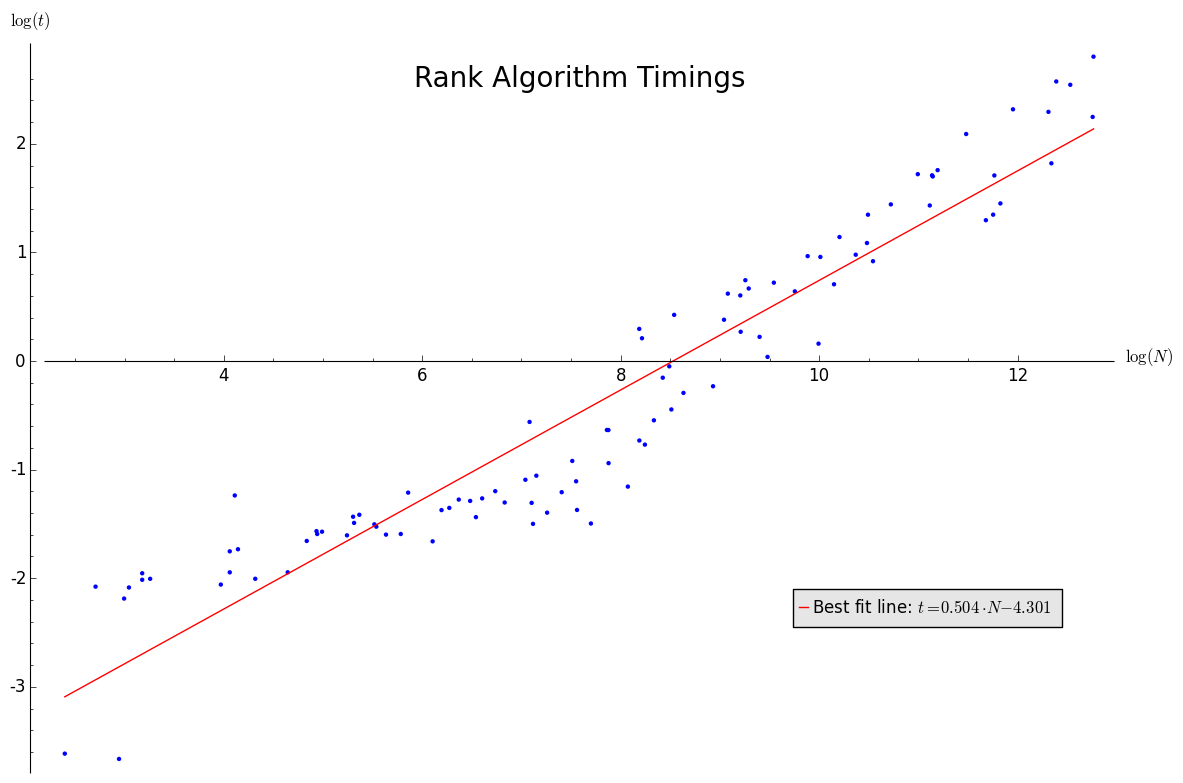
\includegraphics[width=1.0\textwidth]{graphics/rank_algorithm_timings.png}
    \caption{A scatter plot of the time in seconds taken to compute the rank of an elliptic curve using a Sage implementation of Algorithm \ref{algo:compute_rank} (without assuming GRH) vs. conductor, plotted on a log/log scale, for 100 curves drawn randomly from the Cremona database.}
    \label{fig:rank_algorithm_timings}
\end{figure}

For evidence supporting the validity of Theorem \ref{thm:main_theorem}, I wrote a na\"{i}ve implementation of Algorithm \ref{algo:compute_rank} in Sage and collected timings on SageMathCloud of the algorithm's runtime. 100 curves were drawn from the Cremona database according to a log-uniform distribution on their conductors; a log/log scatter plot of timings vs. conductors can be seen in Figure \ref{fig:rank_algorithm_timings} (the algorithm produced the correct output in all cases). \\

The red line in the figure is the best fit straight line, which has slope $0.503$; the predicted slope of $0.5$ is well within the sample error of $0.016$. This is therefore good computational evidence that the runtime of the rank algorithm does indeed scale with $\sqrt{N_E}$.  \\

Using this best fit line, we can make predictions as to how long the algorithm will take to run on curves of larger conductor. For example, the curve of largest known rank is a rank 28 curve found by Elkies (as discussed in \cite{Bob-2011}); it has conductor $\log N_E \sim 325.9$. For this curve we estimate Algorithm \ref{algo:compute_rank} to take roughly $1.1\times 10^{62}$ years, which is about $8\times 10^{51}$ times the age of the universe. \\

Clearly then, the $\softO(\sqrt{N_E})$ time complexity of Algorithm \ref{algo:compute_rank} limits its usefulness when it comes to curves of large rank. For a method that can be used on such curves, see Chapter 5.

\newpage
%%%%%%%%%%%%%%%%%%%%%%%%%%%
\section{The Real Period}\label{sec:real_period}

The real period of a rational elliptic curve $E$ is a measure of the ``size'' of the set of {\it real} points on $E$. \\

Recall that $E(\CC)$, the group of complex points on $E$, is isomorphic via the (inverse of the) Weierstrass $\wp$-function to $\CC$ modulo a lattice under addition; that is, $E(\CC) \simeq \CC/\Lambda$, where $\Lambda = \ZZ\omega_1 + \ZZ\omega_2$, and $\omega_1,\omega_2 \in \CC$.
If $E$ is defined over the real numbers (as rational elliptic curves are), then we may always write $\omega_1$ as being positive real. The second generator $\omega_2$ can be written as being positive imaginary when $E$ has positive discriminant, or in the upper half plane with real part $\frac{\omega_1}{2}$ when $E$ has negative discriminant. [Note: some texts normalize $\omega_2$ to have imaginary part equal to $-\frac{\omega_1}{2}$ when $D_E<0$, as this sometimes makes the presentation more natural. However, for the work below we will always assume that $\Re(\frac{\omega_2}{\omega_1}) = 0$ or $\frac{1}{2}$.] See \cite[Ch. VI]{Sil-1985} and \cite[Ch. I]{Sil-1994} for a more detailed exposition of the complex theory of elliptic curves and elliptic and modular functions respectively.

\begin{definition}\label{defn:real_period}
Let $E/\QQ$ have discriminant $D_E$, and $E(\CC) \simeq \CC/\Lambda$, where $\Lambda = \ZZ\omega_1 + \ZZ\omega_2$ and $\omega_1 \in \RR$. The {\it real period} of $E$ is defined to be
\begin{equation}
\Omega_E = \begin{cases} 2\omega_1 & D_E > 0 \\ \omega_1 & D_E < 0 \end{cases}.
\end{equation}
\end{definition}

We are interested in answering the question: For a curve of a given discriminant, how big and how small can $\Omega_E$ be? Can the real period be arbitrarily small or large, or does it scale in some meaningful way with the discriminant? For our purposes, establishing a lower bound on $\Omega_E$ is what is needed to bound the central leading Taylor coefficient of $\Les$ from below. However, we include the result giving an upper bound on $\Omega_E$, as we find its implication -- that $\Omega_E$ goes to zero as $N_E$ goes to infinity -- an interesting one. \\

First, an upper bound. To this end, we have the following result from the complex theory of elliptic curves:
\begin{proposition}
Let $\Delta(z)$ be the Ramanujan Delta function on the complex upper half plane, i.e.
\begin{equation}
\Delta(z) = q \prod_{n=1}^{\infty} (1-q^n)^{24},
\end{equation}
where $q = e^{2\pi i z}$. Let $E/\CC$ have discriminant $D_E$ and lattice basis $(\omega_1,\omega_2)$ as defined above. Set $z = \frac{\omega_1}{\omega_2}$ (such that $\Im(z) > 0$). Then
\begin{equation}\label{eqn:modular_discriminant}
D_E = \left(\frac{2\pi}{\omega_1}\right)^{12} \Delta\left(z \right).
\end{equation}
\end{proposition}
A proof of the above can be found in Chapter I of \cite{Sil-1994}. Using this result we can readily establish an upper bound on $\Omega_E$:
\begin{proposition}\label{prop:real_period_upper_bound_discriminant}
Let $E/\QQ$ have discriminant $D_E$ and real period $\Omega_E$. Then
\begin{equation}\label{eqn:real_period_upper_bound_discriminant}
\Omega_E < 8.82921517\ldots \cdot (D_E)^{-\frac{1}{12}}.
\end{equation}
\end{proposition}
\begin{proof}
Equation \ref{eqn:modular_discriminant} yields
\begin{equation}
\omega_1 = 2\pi |D_E|^{-\frac{1}{12}} \left| \Delta\left(\frac{\omega_2}{\omega_1}\right)\right|^{\frac{1}{12}}.
\end{equation}
Recall that since $E$ is defined over $\QQ$, we may choose a lattice basis $(\omega_1, \omega_2)$ such that $\omega_1 \in \RR_{+}$ and the real part of $\omega_2$ equals either $0$ or $\frac{\omega_1}{2}$. Thus we may take $z = \frac{\omega_2}{\omega_1}$ to have real part either equal to 0 or $\frac{1}{2}$. Moreover, $\Re(s)=0$ if $D_0>0$ and $\Re(z)=\frac{1}{2}$ if $D_E<0$. See Chapter I of \cite{Sil-1994} for proofs of these statements. \\

Thus $D_E>0$ corresponds to $q = e^{2\pi i z}$ being positive real lying in the open interval $q \in (0,1)$, while $D_E<0$ corresponds to $q \in (-1,0)$. Now $\Delta$ is a cuspidal modular form on $\SL_2(\ZZ)$, so as a function of $q$, $\Delta(q)$ is continuous on $(-1,1)$, zero at the origin, and decaying to zero at $q=-1$ and $q=1$. It must therefore achieve a maximum magnitude on both open intervals $q \in (-1,0)$ and $q \in (0,1)$. \\

The critical points of $\Delta$ have been studied in there own right -- see for example \cite{IJA-2013} and \cite{WoYo-2013}. We see that $\Delta(q)$ has precisely one critical point on each of the intervals $q \in (-1,0)$ and $q \in (0,1)$; these occur at $q = 0.03727681\ldots$ and $q =-0.43929305\ldots$ respectively (corresponding to $z=0.52352170\ldots i$ and $z=\frac{1}{2}+0.13091903\ldots i$ in the upper half plane respectively). At these two values we have $|\Delta(q)|^{\frac{1}{12}}$ equal to $0.70258935\ldots$ and $1.40521323\ldots$ respectively. We conclude that
\begin{equation}
\Omega_E \le 2\pi\cdot 1.40521323\ldots \cdot  |D_E|^{-\frac{1}{12}} = 8.82921517\ldots \cdot |D_E|^{-\frac{1}{12}}.
\end{equation} 
\end{proof}

Note that the real period is {\it not} invariant under isomorphism over $\QQ$. As the elliptic discriminant $D_E$ varies by a twelfth power of an integer as one considers $\QQ$-isomorphic models of $E$, the real period varies by the negative first power of that same integer. This is an immediate consequence of the following statement:
\begin{lemma}
Let $E$ be the global minimal model of a rational elliptic curve, and let $D_E$ and $\Omega_E$ be its discriminant and real period respectively. Let $E\pr$ be isomorphic to $E$ over $\QQbar$, and let $D_{E^{\pr}}$ and $\Omega_{E^{\pr}}$ be defined analogously. Then there exists a $u$ such that  $u^{12}\in \ZZ$, where $D_{E^{\pr}}=u^{12} D_E$ and $\Omega_{E^{\pr}}=\frac{1}{u}\Omega_E$.
\end{lemma}
A proof of the result regarding the discriminant can be found on pages 48-49 of \cite{Sil-1985}; the result regarding the real period follows, for example, from Equation \ref{eqn:modular_discriminant} by chasing through how $D_E$ and $\Omega_E$ vary under $\CC$-isomorphism. \\

Another consequence is that the bound given in Equation \ref{eqn:real_period_upper_bound_discriminant} is optimal, in the sense that the $\frac{1}{12}$ in the negative power of the discriminant cannot be replaced with any larger value. As an explicit example, consider the family of CM elliptic curves given by Weierstrass equations
\begin{equation}
E^d: \;\; y^2 = x^3 - d^2 x,
\end{equation}
for $d \in\ZZ$ positive squarefree. This is just the family of curves related to the congruent number problem, one of the oldest open problems in mathematics (for an excellent treatment on congruent numbers and how they relate to elliptic curves, see \cite{Kob-2012}). Then $E^{d}$ is just the quadratic twist by $d$ (hence the notation) of the curve
\begin{equation}
E: \;\; y^2 = x^3-x,
\end{equation}
which has discriminant 64 and conductor 32. For this family we may actually write down $\Omega_{E^d}$ in terms of a special value of the Gamma function:
\begin{equation}
\Omega_{E^d} = \frac{\Gamma(\frac{1}{4})^2}{\sqrt{2\pi d}}.
\end{equation}
This follows from the fact that $\frac{\omega_2}{\omega_1} = i$ for any of the $E^d$, and that
\begin{equation}
\Delta(i) = \frac{\Gamma(\frac{1}{4})^{24}}{2^{24}\pi^{18}}
\end{equation}
(first shown by Ramanujan in his second notebook -- see \cite{BeZh-1992}). Furthermore, $E^{d}$ has discriminant $D_{E^{d}} = (2d)^6$. So using equation \ref{eqn:modular_discriminant}, for congruent number curves we obtain
\begin{equation}
\Omega_{E^d} = \frac{\Gamma(\frac{1}{4})^2}{\sqrt{\pi}} \cdot (D_{E^d})^{-\frac{1}{12}} = 7.416\ldots \cdot (D_{E^d})^{-\frac{1}{12}}.
\end{equation}
Since $4\pi = 12.566\ldots$ this result conforms with the bound given in Equation \ref{eqn:real_period_upper_bound_discriminant}. It should also be clear from the example above that any family of quadratic twists of a given curve will have the real period scale with the $-\frac{1}{12}$th power of the discriminant. Furthermore, since the $j$-invariant is surjective, we can find $E/\QQ$ with $z=j^{-1}(E)$ arbitrarily close to $\frac{1}{2}+0.13091903\ldots i$, so the constant $8.82921517\ldots$ obtained in Proposition \ref{prop:real_period_upper_bound_discriminant} is also optimal. \\

\begin{corollary}\label{cor:real_period_upper_bound}
For $E/\QQ$ with real period $\Omega_E$ and conductor $N_E$,
\begin{equation}
\Omega_E < 8.82921517\ldots \cdot (N_E)^{-\frac{1}{12}}.
\end{equation}
That is, the real period goes to zero as the conductor of the curve goes to infinity.
\end{corollary}
This follows immediately from Proposition \ref{prop:real_period_upper_bound_discriminant}, as the conductor of an elliptic curve always divides its discriminant. Again, by the same reasoning as before this bound should be optimal. Note that this result is unconditional. \\

Equation \ref{eqn:modular_discriminant} gives us a way to compute the real period of $E$, but it is in general not the most efficient means of doing so (as $z = \frac{\omega_1}{\omega_2}$ must be found by, for example, inverting the $j$-invariant of $E$). Instead, $\omega_1$ may be computed using the (real version of the) Gauss arithmetic-geometric mean. Recall the definition thereof: let $a,b \in \RR_{\ge0}$. Set $a_0 = a$ and $b_0 = b$, and for $n\ge 0$ let $a_{n+1} = \frac{1}{2}(a_{n}+b_{n})$ and $b_{n+1} = \sqrt{a_{n}b_{n}}$. Then $\AGM(a,b)$ is defined to be the common limit of both the $a_n$ and the $b_n$. Moreover, the convergence is quadratic -- precision roughly doubles with every iteration -- and is thus very quick. A deeper exposition of the AGM including a proof of convergence and convergence rate can be found in \cite{Cox-2000}.

\begin{proposition}\label{prop:real_period_by_AGM}
Let $E/\Q$ have minimal Weierstrass equation $y^2 + a_1 xy + a_3 y^2 = x^3 + a_2 x^2 + a_4 x + a_6$. Write the equation in the form
\begin{equation}\label{eqn:weierstrass_with_bn}
\left(y + \frac{a_1x + a_3}{2}\right)^2 = x^3 + \frac{b_2}{4} x^2 + \frac{b_4}{2} x + \frac{b_6}{4} = (x-e_1)(x-e_2)(x-e_3),
\end{equation}
where $e_1,e_2,e_3$ are the 3 complex roots of the polynomial in $x$ on the right hand side, and $b_2$, $b_4$ and $b_6$ are as defined in Section \ref{subsec:notation}.
\begin{enumerate}
\item If $D_E > 0$, then $e_1,e_2,e_3 \in \RR$, so without loss of generality we may order them as $e_3 > e_2 > e_1$. Then
\begin{equation}\label{eqn:omega_D_pos}
\omega_1 = \frac{\pi}{\AGM(\sqrt{e_3-e_1},\sqrt{e_3-e_2})}.
\end{equation}
\item If $D_E < 0$, then the RHS polynomial has only one real root; we may write $e_3 \in \RR$ and $e_1 = \conj{e_2}$. Let $z = \sqrt{e_3-e_1} = s + it$; choose the root such that $s>0$. Then
\begin{equation}\label{eqn:omega_D_neg}
\omega_1 = \frac{\pi}{\AGM(|z|,s)}.
\end{equation}
\end{enumerate}
\end{proposition}
\begin{proof}
Cremona and Cremona-Thongjunthug give good explanations and derivations this formula in \cite{Cre-1997} and \cite{Cre-2013} respectively.
\end{proof}

To get a lower bound on $\Omega_E$ from the above definitions, we will need the following technical result.
\begin{definition}
For a given $E/\QQ$, let 
\begin{equation}
d(E) = \max\set{|e_i - e_j|: \; e_i,e_j \text{ are roots of }4x^3 + b_2  x^2 + 2 b_4 x + b_6, i\ne j}
\end{equation}
be the maximum root separation of the cubic polynomial on the RHS of equation \ref{eqn:weierstrass_with_bn}
(i.e. $b_2, b_4$ and $b_6$ are the $b$-invariants of $E$).
\end{definition}
Observe that for both the positive and negative discriminant cases, the AGM in the denominators in equations \ref{eqn:omega_D_pos} and \ref{eqn:omega_D_neg} is at most $\sqrt{d(E)}$. It is useful therefore to have a bound on the magnitude of $d(E)$ in terms of the $b$-invariants:
\begin{lemma}\label{lem:root_separation_bound}
Given the above setup,
\begin{equation}
d(E) < 2+\frac{1}{2}\max\set{|b_2|,2|b_4|,|b_6|}.
\end{equation}
\end{lemma}
\begin{proof}
We apply Rouche's Theorem on the polynomial $x^3 + \frac{b_2}{4} x^2 + \frac{b_4}{2} x + \frac{b_6}{4}$. Observe that $|\frac{b_2}{4} x^2 + \frac{b_4}{2} x + \frac{b_6}{4}| < |x^3|$ when $|x| < 1+\max\set{\frac{|b_2|}{4},\frac{|b_4|}{2},\frac{|b_6|}{4}}$, so by Rouche's Theorem we must have that any root $e$ of the cubic obeys $|e| <  1+\frac{1}{4}\max\set{|b_2|,2|b_4|,|b_6|}$. The result follows.
\end{proof}

\begin{corollary}[ABC]\label{cor:real_period_time_complexity}
The real period of an elliptic curve can be computed to a specified precision in polynomial time and space in the number of bits of the curve's conductor.
\end{corollary}
\begin{proof}
We see from Proposition \ref{prop:real_period_by_AGM} that $\Omega_0$ can be computed by a) finding the roots of a cubic polynomial related to the Weierstrass equation for $E$, and then b) applying the AGM to a certain simple function of that cubic's roots. \\

Step a) can be achieved in polynomial time in log of the maximum magnitude of the $a$-invariants, which means it can be done in polynomial time in the $c$-invariants. By Modified Szpiro (Conjecture \ref{conj:modified_szpiro}) the conductor of a curve is bounded in magnitude by a polynomial in the $c$-invariants; chaining this all together gives us that step a) can be commuted in time polynomial in $\log N_E$, i.e. sub-polynomial in $N_E$. \\

In step b), Lemma \ref{lem:root_separation_bound} implies that the inputs to the AGM are bounded by a polynomial of the $b$-invariants of $E$, so again by Szpiro they are bounded by a power of $N_E$. The AGM converges quadratically when both the inputs are positive real; therefore it will converge to specified precision with time bounded by a polynomial of $\log N_E$. Thus altogether we see that the real period can be computed to a given precision with time polynomial in $\log N_E$, i.e. sub-polynomial in $N_E$ itself.
\end{proof}

The take-away from the above result is that computing the real period is quick, and will never be the computational bottleneck when it comes to running Algorithm \ref{algo:compute_rank}. \\

\begin{corollary}[S.]\label{ineq:Omega_bn_bound}
Let $E/\Q$ have (not necessarily minimal) Weierstrass equation \\
$y^2 + a_1 xy + a_3 y^2 = x^3 + a_2 x^2 + a_4 x + a_6$ have real period $\Omega_E$, and define $b_2$, $b_4$ and $b_6$ as at the beginning of section \ref{sec:defs_background}. Then
\begin{equation}
\Omega_E > \frac{\alpha \pi}{\sqrt{1+\frac{1}{4}\max\set{|b_2|,2|b_4|,|b_6|}}},
\end{equation}
where $\alpha = 1$ if $E$ has positive discriminant and $\frac{1}{2}$ if $E$ has negative discriminant.
\end{corollary}
\begin{proof}
This follows immediately from the definition of $\Omega_E$ given in Proposition \ref{prop:real_period_by_AGM} and Lemma \ref{lem:root_separation_bound}.
\end{proof}

Again, this bound is optimal in the sense that the square root sign in the denominator cannot be replaced with any smaller exponent. To see this, consider the family of elliptic curves
\begin{equation}
E_n: \;\; y^2 = x^3 - (nx-1)^2.
\end{equation}
For a given $n$, $E_n$ has $b_2,b_4$ and $b_6$ equal to $-4n^2,4n$ and $-4$ respectively.

The polynomial $x^3 + \frac{b_2}{4} x^2 + \frac{b_4}{2} x + \frac{b_6}{4} = x^3 -n^2 x^2 + 2n x - 1$ has a single root at $n^2 - O(\frac{1}{n})$ and two roots very close to the origin with magnitude $O(\frac{1}{n})$. Hence the real period for $E_n$ is
\begin{equation}
\Omega_{E_n} = \frac{2\pi}{n} + O\left(\frac{1}{n}\right).
\end{equation}

On the other hand, for a given $n$
\begin{equation}
1+\frac{1}{4}\max\set{|b_2|,2|b_4|,|b_6|} = 1+n^2.
\end{equation}
for $n\ge 2$. So for this family of curves the lower bound given by inequality \ref{ineq:Omega_bn_bound} is $\frac{\pi}{\sqrt{1+n^2}}$. Since $\Omega_{E_n}$ asymptotes to twice this value, it is clear that the bound would be violated for sufficiently large $n$ if the square root were replaced with a smaller power. \\

Finally, if we assume the Szpiro conjecture, Corollary \ref{ineq:Omega_bn_bound} allows us to the real period of a minimal model of $E$ from below in terms of that curve's conductor. We will invoke a slight reformulation of Modified Szpiro (Conjecture \ref{conj:modified_szpiro}): Suppose the minimal short Weierstrass model of $E$ is $y^2 = x^3+Ax+B$, i.e. there does not exist any prime $p$ such that $p^4|A$ and $p^6|B$. Then for any $\epsilon>0$ there is a constant $K_{\epsilon}$ independent of $E$ such that
\begin{equation}
\max\set{|A|^3,|B|^2} \le K_{\epsilon}\cdot (N_E)^{6+\epsilon}.
\end{equation}
(Since for a curve in short Weierstrass form $c_4 = -48A$ and $c_6=-864B$, we see that the above statement and Modified Szpiro are equivalent). Using this, we obtain the following:
\begin{theorem}[ABC]
\label{thm:real_period_lower_bound}
Let $E$ have conductor $N_E$, and let $\Omega_E$ be the real period of a minimal model of $E$. Then, assuming ABC, for any $\epsilon>0$ there is a constant $K_{\epsilon}$ independent of $E$ such that 
\begin{equation}
\Omega_E > K_{\epsilon} \cdot (N_E)^{-\frac{3}{2}-\epsilon}.
\end{equation}
\end{theorem}
\begin{proof}
Let $E$ be given by its minimal short Weierstrass equation $y^2 = x^3+Ax+B$. $E$ then has $b$-invariants $b_2=0$, $b_4 = 2A$ and $b_6 = 4B$, so by Lemma \ref{ineq:Omega_bn_bound} the real period of $E$ obeys
\begin{equation}\label{eqn:Omega_bound_short_weierstrass}
\Omega_E > \frac{\pi}{2\sqrt{1+\max\set{|A|,|B|}}}.
\end{equation}
Now by the aforementioned version of Szpiro, for any $\epsilon>0$ we have
\begin{align*}
\sqrt{1+\max\set{|A|,|B|}} &<  1 + \max\set{|A|^2,|B|^2}^\frac{1}{4} \\
&\le 1 + \max\set{|A|^3,|B|^2}^\frac{1}{4} \quad\quad\mbox{since $A \in \ZZ$} \\
&\le 1 +\left[K_{\epsilon} (N_E)^{6+\epsilon} \right]^\frac{1}{4} \\
\Longrightarrow \sqrt{1+\max\set{|A|,|B|}} &< K_{\epsilon} (N_E)^{\frac{3}{2}+\epsilon},
\end{align*}
where to achieve the last line we absorb 1 into $K$ and relabel as necessary to account for the $\frac{1}{4}$th power, and relabel $\frac{\epsilon}{2} \mapsto \epsilon$. Again, after absorbing the factor of $\frac{\pi}{2}$ into $K$ in equation \ref{eqn:Omega_bound_short_weierstrass}, the result follows.
\end{proof}

\begin{figure}[!ht]
    \centering
    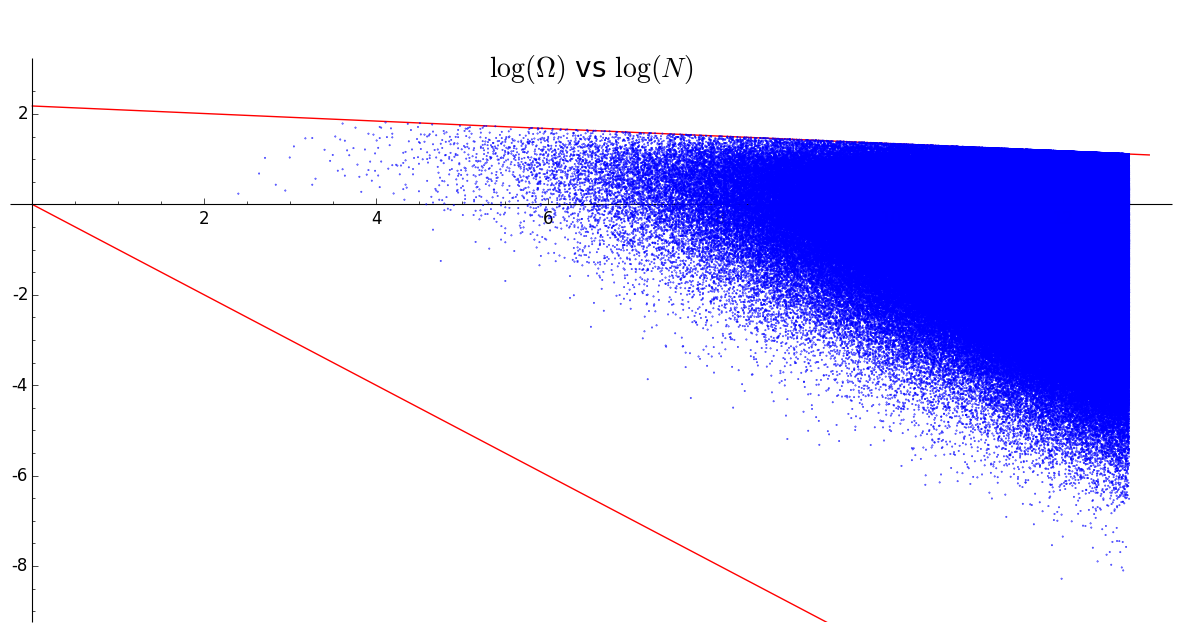
\includegraphics[width=0.92\textwidth]{graphics/real_periods_vs_conductors_loglog}
    \caption{A scatter plot of $\log \Omega_E $ on the vertical axis vs. $\log N_E$ on the horizontal axis, for all curves up to conductor 350000. The upper red line is the proven upper bound $\Omega_E < 8.82921517\ldots \cdot (N_E)^{-\frac{1}{12}}$, which can be seen to be sharp. The lower red line corresponds to the bound $\Omega_E > (N_E)^{-1}$. Empirically this appears to hold easily, lending credence to the validity of the weaker assertion in Conjecture \ref{conj:Omega_lower_bound_explicit}.}
    \label{fig:real_period_vs_conductor_loglog}
\end{figure}

Thankfully, we do not need to assume a specific value of $K_{\epsilon}$ for a given $\epsilon$ for Theorem \ref{thm:main_theorem} to hold. However, empirical data suggests that for $\epsilon=\frac{1}{2}$ we can easily get away by choosing $K = 1$. We formalize this with the following conjecture:
\begin{conjecture}\label{conj:Omega_lower_bound_explicit}
Let $E$ have conductor $N_E$, and let $\Omega_E$ be the real period of a minimal model of $E$.Then 
\begin{equation}
\Omega_E > (N_E)^{-2}.
\end{equation}
\end{conjecture}

\newpage
%%%%%%%%%%%%%%%%%%%%%%%%%%%
\section{The Regulator}

To define the regulator of a rational elliptic curve, we must first define the na\"ive logarithmic height, N\'eron-Tate canonical height and the N\'eron-Tate pairing on points on $E$. \\

Let $E$ be an elliptic curve over $\QQ$ and $P \in E(\QQ)$ a rational point on $E$. The {\it na\"ive logarithmic height} of $P$ is a measure of the size' of the coordinates of $P$. 
\begin{definition}
Define $h(\cO) = 0$. For $P\ne \cO$, we may write $P = (x,y) \in \QQ^2$, with $x = \frac{a}{b}, a,b \in \ZZ$, $b>0$ and $\gcd(a,b) = 1$. We then define the na\"ive height of $P$ to be
\begin{equation}
	h(P) := \max\set{\log|a|,\log|b|}.
\end{equation}
\end{definition}
If you compute the na\"ive heights of a number of points on an elliptic curve, you'll notice that the na\"ive height function is ``almost a quadratic form'' on $E$. That is $h(nP) \sim n^2 h(P)$ for integers $n$, up to some constant that doesn't depend on $P$. We can turn $h$ into a true quadratic form as follows:

\begin{definition}
The {\it N\'eron-Tate height} height function $\hat{h}: E(\QQ) \to \RR$ is defined as
\begin{equation}
	\hat{h}(P) := \lim_{n \to \infty} \frac{h(2^n P)}{(2^n)^2},
\end{equation}
where $h$ is the na\"ive logarithmic height defined above.
\end{definition}

\begin{theorem}[N\'eron-Tate]
N\'eron-Tate defines a canonical quadratic form on $E(\QQ)$ modulo torsion. That is,
\begin{enumerate}
	\item For all $P,Q \in E(\QQ)$,
	\begin{equation}
		\hat{h}(P+Q) + \hat{h}(P-Q) = 2\left[ \hat{h}(P) + \hat{h}(Q)\right],
	\end{equation}
	i.e. $\hat{h}$ obeys the parallelogram law;
	\item For all $P \in E(\QQ)$ and $n \in \ZZ$,
	\begin{equation}
		\hat{h}(nP) = n^2 \hat{h}(P).
	\end{equation}
	\item $\hat{h}$ is even, and the pairing $\langle\;,\;\rangle: E(\QQ)\times E(\QQ) \to \RR$ by
	\begin{equation}
		\langle P,Q \rangle = \frac{1}{2}\left(\hat{h}(P+Q) - \hat{h}(P) - \hat{h}(Q)\right)
	\end{equation}
	is bilinear;
	\item $\hat{h}(P) = 0$ iff $P$ is torsion;
	\item We may replace $h$ with another height function on $E(\QQ)$ that is ``almost quadratic'' without changing $\hat{h}$.
\end{enumerate}
\end{theorem}

For a proof of this theorem and elaboration on the last point, see \cite[pp. 227-232]{Sil-1985}.

\begin{definition}
The {\it N\'eron-Tate pairing} on $E/\QQ$ is the bilinear form $\langle\;,\;\rangle: E(\QQ)\times E(\QQ) \to \RR$ by
	\begin{equation}
		\langle P,Q \rangle = \frac{1}{2}\left(\hat{h}(P+Q) - \hat{h}(P) - \hat{h}(Q)\right).
	\end{equation}
\end{definition}
Note that this definition may be extended to all pairs of points over $\QQbar$, but the definition above suffices for our purposes. \\

If $E(\QQ)$ has rank $r$, then $E(\QQ)/E_{\text{tor}}(\QQ) \hookrightarrow \RR^r$ as a rank $r$ lattice via the height pairing map. Specifically, if $\set{P_1,\ldots, P_r}$ is a basis for $E(\QQ)$ modulo torsion, then we send $Q \in E(\QQ)$ to the vector $\left( \langle Q,P_1 \rangle, \ldots, \langle Q,P_r \rangle \right)$. Note that the image of a given point under this embedding obviously depends on the choice of basis. However, any two lattices comprising the image of $E(\QQ)$ using two different basis choices are isomorphic, and thus always have the same covolume.

\begin{definition}
The {\it regulator} $\Reg_E$ of $E/\QQ$ is the covolume of the lattice that is the image of $E(\QQ)$ under the above pairing map. That is, if $\set{P_1,\ldots,P_r}$ generates $E(\QQ)$, then
\begin{equation}
	\Reg_E = \det\left(\langle P_i,P_j\rangle \right)_{1 \le i,j \le r},
\end{equation}
where $\left(\langle P_i,P_j\rangle \right)_{1 \le i,j \le r}$ is the matrix whose $(i,j)$th entry is the value of the pairing $\langle P_i,P_j\rangle$. If $E/\QQ$ has rank zero, then $\Reg_E$ is defined to be 1.
\end{definition}
Note that for any $P \in E(\QQ)$, $\langle P, P \rangle = \hat{h}(P)$. Thus the regulator of any rank 1 curve is just the smallest height of a non-torsion point on that curve. \\

Loosely, the regulator measures the ``density'' of rational points on $E$: positive rank elliptic curves with small regulators have many points with small coordinates, while those with large regulators have few such points.\\

There are conjectural bounds on how large a curve's regulator can be in terms of its conductor -- see for example Conjecture 6.3 in Lang's Survey of Diophantine Geometry \cite[p. 99]{Lang-1997}. This is a topic we hope to investigate more fully future work, but the question that is relevant to this thesis is not how large the regulator can be, but how small. Specifically, given $E/\QQ$ with (minimal) discriminant $D_E$, what is the smallest $\Reg_E$ can be as a function of $D_E$?

This is an open question. However, recall Lang's Height Conjecture (Conjecture 1.4 in \cite[pp. 73-74]{Lang-1997}):
\begin{quotedconjecture}{\ref{conj:Lang}}
Let $E/\QQ$ have minimal discriminant $D_E$. There exists an absolute constant $M_0 >0$ independent of $E$ such that any non-torsion point $P \in E(\QQ)$ satisfies
\begin{equation}
\hat{h}(P) \ge M_0 \log |D_E| .
\end{equation}
\end{quotedconjecture}
That is, the minimum height of a non-torsion point on $E$ scales with the log of the absolute value of the curve's minimal discriminant. Hindry and Silverman in \cite{HiS-1988} show that the ABC conjecture implies Lang's height conjecture and, better yet, gives an explicit lower bound on $M_0$:
\begin{equation}
M_0 \ge 6\times 10^{-11}.
\end{equation}
The bound was further improved  by Elkies (albeit still contingent on ABC) in the early 2000s \cite{Elk-2006} to
\begin{equation}
M_0 \ge 3.9479\times 10^{-5}.
\end{equation}
Note that Theorem \ref{thm:main_theorem} requires the assumption of ABC for results regarding the real period of $E$; quoting the above result therefore requires no further unproven results. \\

There is general agreement in the literature is that the value of $M_0$ above is not optimal; however, there is no strong consensus as to how much larger $M_0$ could be. A survey by Elkies \cite{ElSt-2002} reveals 54 known cases of points $P$ on curves over $\QQ$ where $\hat{h}(P) < \frac{1}{100}$, and the largest value of $\hat{h}/\log|D_E|$ is $\sim 8.46 \times 10^{-5}$, achieved by a point on a curve of conductor $N=3476880330$. Given the evidence in this and other compiled data, it seems quite likely that there are as-yet undiscovered instances of points with low height driving the observed lower bound down closer to the value of $3.9479\times 10^{-5}$. \\

One can therefor make the more conservative following observation:
\begin{corollary}[ABC]\label{conj:point_height_lower_bound}
There exists an absolute constant $M_1 >0$ independent of $E$ such that any non-torsion point $P$ on any elliptic curve $E(\QQ)$ satisfies
\begin{equation}\label{eqn:Elkies_height_lower_bound}
\hat{h}(P) \ge M_1 .
\end{equation}
\end{corollary}
The smallest absolute point height found in the aforementioned survey by Elkies is $\hat{h}(P) = 8.914\times 10^{-3}$, achieved by the point $P = (7107,-602054)$ and its negative on the curve with Cremona label {\tt 3990v1}, given by the equation $E: y^2+xy+y=x^3+x^2-125615x+61201397$. (note that the Elkies' table uses a slightly different definition of height, equal to half the value of the height as defined above). One can see in this table that the known points of smallest height all belong to curves with small conductor, so it is perhaps more believable that this is indeed the point of smallest height on any rational elliptic curve -- for such a point is guaranteed to exist, assuming ABC. \\

Even though the Elkies bound above would seem so small as to be  of limited use in practical applications, we can use it to bound a curve's regulator from below in terms of an inverse power of its conductor. For this we will need the following geometric lemma:
\begin{lemma}\label{lem:covolume_lower_bound}
Let $L$ be a lattice in $\RR^r$ with covolume $V_L$. If $h$ is the minimum nonzero vector length in $L$, then
\begin{equation}
V _L \ge \left(\frac{\sqrt{\pi}}{2}\cdot h\right)^{r} \cdot \frac{1}{\Gamma(1+\frac{r}{2})},
\end{equation}
where $\Gamma(s)$ is the usual Gamma function on $\CC$.
\end{lemma}
\begin{proof}
Recall Minkowski's Theorem: Let $L$ be a lattice in $\RR^r$ with covolume $V_L$, and let $S$ be a convex symmetric subset of $\RR^r$ with volume $\Vol(S)$. If $\Vol(S)>2^r \cdot V_L$, then $S$ contains a nonzero element of $L$ -- see \cite[p. 80]{st-2012} for a proof. \\

So let $S = B(0,h)$, i.e. the open ball of radius $h$ centered at the origin, where $h$ is the minimum nonzero vector length in $L$. By construction $S$ contains no nonzero lattice elements, so by Minkowski's theorem we must have that
\begin{equation}
\Vol(S) \le 2^r V_L.
\end{equation}
The volume of the $r$-sphere with radius $L$ is given by
\begin{equation}
\Vol(S) = \frac{\pi^{\frac{r}{2}}}{\Gamma(1+\frac{r}{2})} \cdot h^r;
\end{equation}
combining the above two statements and solving for $V_L$ completes the result.
\end{proof}

With the above lemma we can then prove the following:
\begin{theorem}[BSD, ABC, (GRH)]\label{thm:regulator_lower_bound}
Let $E/\QQ$ have conductor $N_E$. Assuming BSD and ABC, we have that
\begin{equation}
\Reg_E \ge 4.36 \times 10^{-6} \cdot (N_E)^{-3.86} \cdot \frac{1}{\Gamma(1.8+0.25 \log N_E)}.
\end{equation}
If one further assumes GRH, then one has the improved bound
\begin{equation}
\Reg_E \ge 2.11 \times 10^{-2} \cdot (N_E)^{-2.47} \cdot \frac{1}{\Gamma(1.25+0.16 \log N_E)}.
\end{equation}
\end{theorem}
\begin{proof}
For curves of conductor $\le 350000$, we consulted Cremona's tables and verified numerically that the above statements. Thus without loss of generality we may assume $D_E \ge N_E > 350000$. Hence for any point $P \in E(\QQ)$, by Conjecture \ref{conj:Lang} and the Elkies' bound in Equation \ref{eqn:Elkies_height_lower_bound} we have that
\begin{equation}
\hat{h}(P) \ge 3.9479\times 10^{-5} \cdot \log |D_E| \ge 6\times10^{-11} \cdot \log(350000) = 5.0397 \times 10^{-4}.
\end{equation}
Let $h = 5.0397 \times 10^{-4}$, and let $L$ be the rank $r$ lattice that is the image of $E(\QQ)$ under the height pairing map (for a given choice of basis of $E(\QQ)$), where $r$ is the rank of $E$. It follows that any nonzero vector in $L$ has length at least $h$. Thus by Lemma \ref{lem:covolume_lower_bound} we must then have that
\begin{equation*}
\Reg_E \ge \left(\frac{\sqrt{\pi}}{2}\cdot h\right)^{r} \cdot \frac{1}{\Gamma(1+\frac{r}{2})}.
\end{equation*}
By BSD, the algebraic and analytic rank are equal, so we have that
\begin{equation}
r < a\log N_E + b,
\end{equation}
where by Corollary \ref{cor:logderiv_rank_bound} we may take $a=0.5, b=1.6$ if we aren't assuming GRH, and by Corollary \ref{cor:better_an_bound} $a=0.32, b=0.5$ if we are. Thus
\begin{align*}
\Reg_E &\ge \left(\frac{\sqrt{\pi}}{2}\cdot h\right)^{a \log N_E + b} \cdot \frac{1}{\Gamma\left(1+\frac{a \log N_E + b}{2}\right)} \\
&= \left(\frac{\sqrt{\pi}}{2}\cdot h\right)^{b} \cdot \left(N_E\right)^{a\log \left(\frac{\sqrt{\pi}}{2}\cdot h\right)} \cdot \frac{1}{\Gamma\left((1+\frac{b}{2})+\frac{a}{2} \log N_E \right)}.
\end{align*}
[Note that replacing $r$ with $a\log N_E +b$ inside the Gamma factor is only valid in the region where the Gamma function is monotonically increasing, i.e. for $a\log N_E + b \ge 1$. However, we are in this case in both the non-GRH and GRH versions of the proof, since we are assuming $N_E > 350000$.] \\

Substituting the respective values of $a$ and $b$ and simplifying produces the two inequalities stated in the theorem.
\end{proof}
There are a few things worth pointing out about this result. Firstly, the Gamma factor means that the proven lower bound on the regulator eventually decreases more rapidly than any negative power of the conductor. However, since $\Gamma(s) = O(e^{s\log s})$, we see that $\Gamma\left((1+\frac{b}{2})+\frac{a}{2} \log N \right) = O(N^{c\log\log N})$ for some constant $c$. That is, the exponent in the negative power of $N_E$ coming from the Gamma factor grows, albeit very slowly. \\

Note that (without assuming GRH), the number of bits extra precision needed in Algorithm $\ref{algo:compute_rank}$ required to compensate for the Gamma factor is $\log_2(\Gamma(1.8+0.25\log N_E))$. Even though this quantity grows faster than $\log N_E$, the constant in front of $\log N_E$ inside the Gamma factor is small enough that for all practical purposes the number of bits precision needed to account for the Gamma factor grows linearly with log of the conductor over the range of conductors for which the rank algorithm is practical. For example, when $N_E=350000$ the number of extra bits precision needed to accommodate for the Gamma factor is just 5 (even without assuming GRH). And even for $N_E = 10^{20}$ -- which is about the upper limit for what is practical on modern architecture -- the number of extra bits needed is 30. Either way, the number of bits needed to account for the regulator isn't an issue in any way since the computational bottleneck in the rank algorithm is the $\sqrt{N_E}$ dependence coming from evaluating $L_E(s)$, which grows faster than any power or $\log N_E$. \\

Also note that the first step in the proof -- manual verification for all curves below conductor $35000$ --  isn't strictly necessary; it only improves the constants in the bounds by a small amount. However, it serves to highlight that the power of $N_E$ in the two bounds can theoretically be improved further by exhaustively checking all curves up to a higher conductor bound. If, for example, we believe that $8.914\times 10^{-3}$ is a global minimum point height over all rational elliptic curves, then (assuming GRH) we would instead get
\begin{equation}
\Reg_E \ge 8.89 \times 10^{-2} \cdot (N_E)^{-1.55} \cdot \frac{1}{\Gamma(1.25+0.16 \log N_E)}.
\end{equation}
Even so, we do {\it not} expect either bound to be anywhere close to optimal; almost certainly more careful analysis could further reduce the negative exponent of $N$ or increase the size of the constant in front of it -- or better yet, eliminate the Gamma factor. In practice, we see the smallest regulators tend to {\it grow} with conductor, further highlighting that the above bound is rather crude. However, the statement in Theorem \ref{thm:regulator_lower_bound} is good enough for our purposes: it will help establish that the central leading coefficient of $\Les$ cannot be exponentially small in $N_E$. \\

We invite the interested reader to improve upon this result, and thus ultimately speed up the runtime of Algorithm \ref{algo:compute_rank}. 